\section{Grafikk}

\subsection{Computer Graphics}
Å lage et rasterbilde fra en scene. \\
Scene $\rightarrow$ Computer Graphics $\rightarrow$ Raster image

\subsubsection{Visualisering}
Bruke en visuell presentasjon av data for å øke forståelse. \\
Data Set $\rightarrow$ Visualization $\rightarrow$ Model 

\subsubsection{Modellering}
Teknikker for å representere grafiske objekter.\\
Model$\rightarrow$ Graphics Pipeline $\rightarrow$ Image

\subsubsection{Image buffer}
2-dimensjonalt array med W x H, hvor hver piksel har et gitt antall bits (for å representere en farge/intensitet). I minnet er disse lineære.

Et dobbeltbuffer er at man har to buffre (fyller opp det ene, viser det andre).

\subsubsection{Color look up table}
Et ekstra nivå med indireksjon, der fargene er lagret i en tabell ved siden av, og image buffer inneholder index til denne tabellen.

\subsubsection{Hardware}
Grafikkort har gjerne Z-buffer og lar seg programmere med shaders (vertex og fragment).

\subsection{Rasterisering}
Konvertering av 2D-primitiver til diskrete pikselrepresentasjoner. I utgangspunktet er kompleksiteten for rasterisering $O(Pp)$ der P er antall primitiver og p er antall piksler.

\subsubsection{Midtpunkt og nabolag}
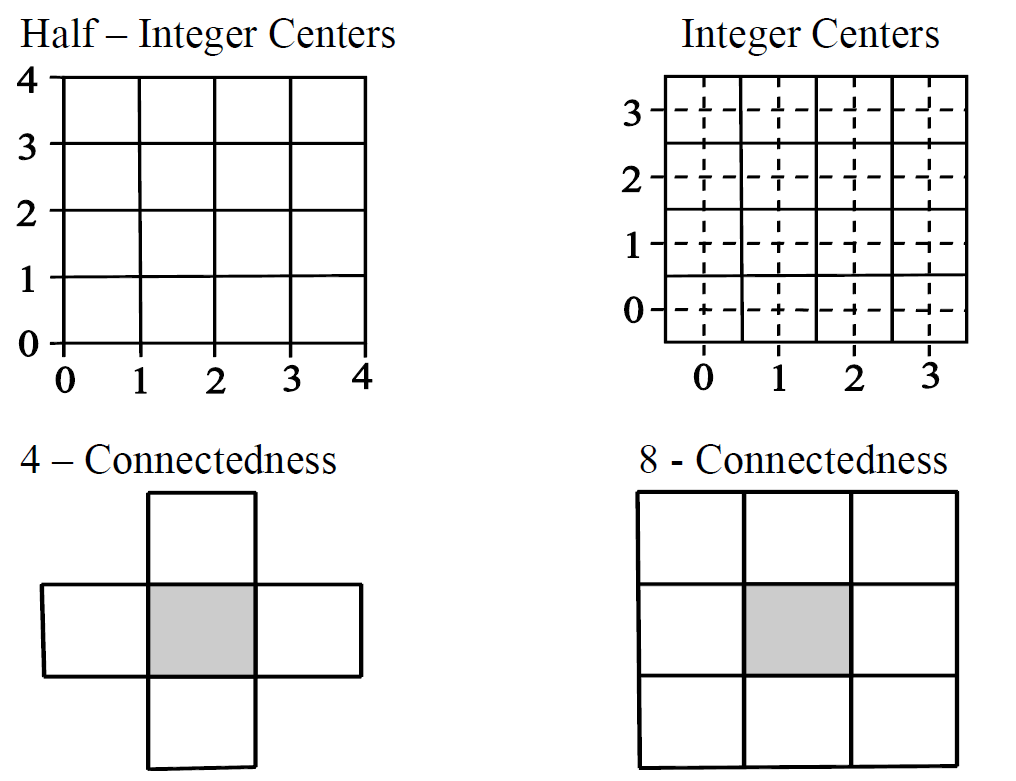
\includegraphics[width=\textwidth]{Bilder/centers.png}

\subsection{Rasteriseringsalogritmer for linjer}
Må dele opp i oktanter. Det er lett å konvertere fra én oktant til en annen.
\\ 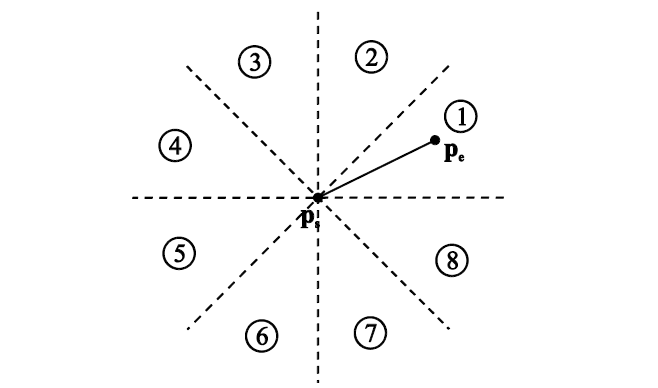
\includegraphics[width=\textwidth]{Bilder/oct.png}

\subsubsection{Suboptimal}
I en suboptimal algoritme akkumulerer man feil med stigningstallet. For hver x-verdi man skriver får man en ny feil i y-retningen. Dersom denne feilen er større enn 0.5, legger man til én på y, og trekker én fra feilen. Gjelder i 1. kvadrant.

\begin{lstlisting}
while(x<=xe) {
    x +=1;
    e +=dy/dx; #dy/dx = s
    if(e >= 0.5) {
        y += 1
        e -= 1
    }
}
\end{lstlisting}

Dette inneholder for mye flyttalsaritmetikk, så hvis man ganger alt som har med bestemmelsesverdier å gjøre med dx, får man bare heltall.

\begin{lstlisting}
while(x<=xe) {
    x +=1;
    e +=dy;
    if(e >= floor(0.5*dx)) {
        y += 1
        e -= dx
    }
}
\end{lstlisting}

Ved å sette e til -0.5*dx i starten, er det enklere å se om man skal hoppe, siden man bare trenger å sjekke om  $e>=0$.

\subsection{Rasteriseringsalgoritmer for sirkler}
En sirkel har en 8-veis-symmetri. Hver enkelt piksel settes til alle permutasjoner av [x, -x] og [y, -y]. Beskrevt algoritme tar utgangspunkt i oktant 2 og dekrementerer y.

Bruk en sirkelfunksjon med sentrum i (0, 0.5) (vet ikke hvorfor):
\begin{equation}
    c(x, y) = x^2 +(y-0.5)^2 - r^2 = 0
\end{equation}

Vi begynner på toppen av sirkelen og går med klokken. Siden x=0 her og vi har en radius på r, får vi da en startfeil:
\begin{equation}
    c(0, r) = (r - 0.5)^2 - r^2 = 0.25 - r \approx -r
\end{equation}
Vi fjerner 0.25 siden vi ønsker å operere med heltall. \\
Vi bruker endelige differanser for endring i x og y, henholdsvis
\begin{equation}
    c(x+1,y)-c(x,y) = 2x+1
\end{equation}

\begin{equation}
    c(x,y+1)-c(x,y) = -2y + 2
\end{equation}

Dette er de to potensielle stegene vi kan få i algoritmen.

\begin{lstlisting}
x=0; y=r; e=-r;
while (x <= y) {
    set8pixels(x, y, c);
    e += 2*x + 1; #fremoverdifferansen til x
    x += 1;
    if(e >= 0) {
        e -= 2*y + 2; #fremoverdifferansen til y
        y -= 1;
    }
}
\end{lstlisting}

\subsection{Point in polygon}
\begin{itemize}
    \item Parity test: Hvor mange kanter krysser jeg?
    \item Winding test: Følg kanten og snurr rundt. Odde er innefor, par er utenfor.
    \item For konvekse polygoner: Sett samme retning på alle kanter, sett inn punktkoordinatene i alle linjelikningene og sjekk om alle har samme tegn.
\end{itemize}

\subsection{Polygon rasterization}
\subsubsection{Enklest}
Regn ut $I(x,y)$, alle punkter der scanline og kanter i polygonet krysser. Sorter etter $(y,x)$, lag spans mellom pikslene i mellom.
\\ 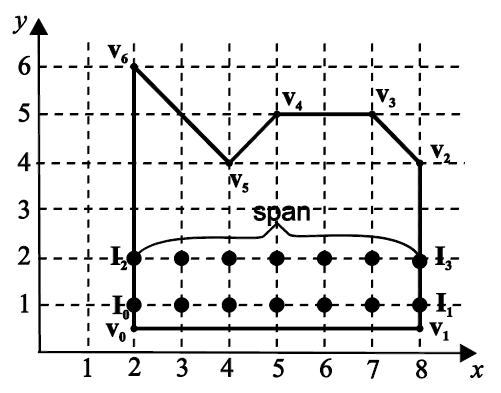
\includegraphics[width=\textwidth]{Bilder/scanline.png}
Her forekommer det noen problemer med noder som havner på skannelinjene. Løsning:
\begin{itemize}
    \item Lukk linjer ved $y_{min}$ og åpne de ved $y_{max}$.
    \item Ignorer horisontale kanter.
\end{itemize}
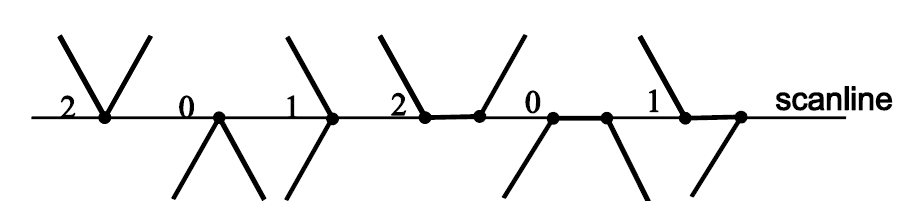
\includegraphics[width=\textwidth]{Bilder/scanline2.png}

\subsubsection{Scanline Polygon Rasterization ALgorithm}
Please, kan noen forklare meg denne?

\subsubsection{Triangle rasterization}
Enkleste: Ta bounding box og bruk "point in polygon test" på alle piksler i denne boundingboksen. Point in polygon er enkelt med en trekant (konveks), bare sjekk om alle linjer har samme fortegn. \\
Vanskeligere: Edge walking. Bruk Bresenham per linje. Synkroniser algoritmene slik at de får samme y- eller x-verdier.

\subsubsection{Area Filling}
Man kan brke en rekursiv floodfill-algoritme som fyller ut farge fra et seeding-punkt.
    
\subsection{Anti-aliasing}
Dette skjer fordi piksler ikke er matematiske punkter men små arealer. Uønskede effekter:
\begin{itemize}
\item Jagged appearance of object silhouettes
\item Improperly rasterized small objects
\item incorrectly rasterized detail
\end{itemize}
\subsubsection{Pre-filtering}
Dette består av å få ut høye frekvenser før sampling, og regne ut totalt bidrag.

\paragraph{Catmull's algorithm}
Klipp i hver piksel, og regn på hvor mye areal fra hver polygon som er synlig. Juster farge deretter.

\paragraph{Anti-aliased Line Rasterization}
En linje som spenner over to piksler ønsker:
\begin{itemize}
    \item Topp-piksel har farge proposjonalt med A2.
    \item Bunnpikser har farge proposjonalt med 1-A1.
\end{itemize}
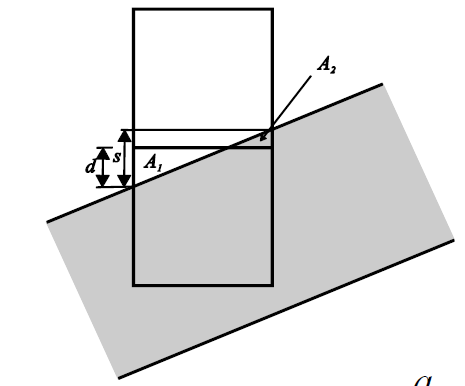
\includegraphics[width=\textwidth]{Bilder/aalr.png}

\subsubsection{Post-filtering}
Virutelt bilde. feks. nidoble antall piksler , regne ut snittet av 3x3-ruter og legge dette i én piksel. Dette blir bedre om man bruker konvolusjonsfiltre (mer vekt på piksler i sentrum).
\\Adaptiv: Bedre sampling ved høye frekvenser.
\\Stokastisk: Lage støy av anti-aliasing.
    

\subsection{Clipping}\label{subsection:clipping}
\subsubsection{Cohen-Sutherland}
Dette er en algoritme for å klippe linjer slik at de passer inn i et vindu. For hvert endepunkt i linjene du klipper, definér fire bits:
\begin{enumerate}
    \item y\textgreater y\textsubscript{max} ? 1 : 0
    \item y\textless y\textsubscript{min} ? 1 : 0
    \item x\textgreater x\textsubscript{max} ? 1 : 0
    \item x\textless x\textsubscript{min} ? 1 : 0
\end{enumerate}

\paragraph{Triviell aksept}
To endepunkter er fullstendig på innsiden dersom: 
\begin{math} c\textsubscript{1} \vee c\textsubscript{2} = 0000 \end{math}

\paragraph{Triviell forkastning}
To endepunkter er fullstendig på utsiden dersom:
\begin{math} c\textsubscript{1} \wedge c\textsubscript{2} \neq 0000 \end{math} \\

Alle andre linjer klippes i to og behandles rekursivt til alle er helt inni eller utenfor.

\subsubsection{Skala}
Legger på et ekstra bit ekstra informasjon per vertex når den klipper. Den ekstra bitten er 1 dersom fortegnet til linjen den klippes med er positiv. Den kan regne seg frem til hva som er på innsiden og hva som er på utsiden ved å gjøre en enkel sjekk.

\subsection{Liang-Barsky}
Gjør om linjene til parameteriserte former. Merk at dette alltid på være tilfelle:
\begin{equation}
x_{min} \le x_1 + t\Delta x \le x_{max}
\end{equation}
\begin{equation}
y_{min} \le y_1 + t\Delta y \le y_{max}
\end{equation}

Dette fører til:
\begin{equation}
-t\Delta x \le x_1 - x_{min}
\end{equation}
\begin{equation}
t\Delta x \le x_{max} - x_1
\end{equation}
\begin{equation}
-t\Delta x \le y_1 - y_{min}
\end{equation}
\begin{equation}
t\Delta x \le y_{max} - y_1
\end{equation}

Ut ifra dette kan vi få punktsett $(p_i,q_i)$ fordi alle er på formen $t p_i \le q_i$.
\begin{equation}
    (p_1, q_1) = (-\Delta x, x_1 - x_{min})
\end{equation}
\begin{equation}
    (p_2, q_2) = (\Delta x, x_{max} - x_1)
\end{equation}
\begin{equation}
    (p_3, q_3) = (-\Delta y, y_1 - y_{min})
\end{equation}
\begin{equation}
    (p_4, q_4) = (\Delta y, y_{max} - y_1)
\end{equation}

Hver av disse tuplene brukes på henholdsvis venstre, høyre, nedre og øvre kant av klipperammen. For å regne ut hvor linjen går inn, tar man maks av alle ${q_i \over p_i}$ der $p_i$ er mindre enn null. $t_{in}$ kan heller ikke være mindre enn null. For å regne ut $t_{out}$ tar man minste verdi av ${q_i \over p_i}$ der $p_i$ er større enn null. $t_{out}$ kan heller ikke være større enn 1.

\begin{equation}
    t_{in} = max(\{{q_i \over p_i} | p_i < 0, i:1..4\} \cup \{0\})
\end{equation}

\begin{equation}
    t_{out} = min(\{{q_i \over p_i} | p_i > 0, i:1..4\} \cup \{1\})
\end{equation}

Hvis $t_{out} \ge t_{in}$ bruker man disse verdiene for å få nye start- og stoppunkter. Hvis ikke, er linjen utenfor.


\subsubsection{Sutherland-Hodgman}
Klipping av polygon i et annet konveks polygon. Denne algoritmen har $m$ steg som tilsvarer $m$ kanter i klippepolygonet. Klipp polygonet for hver kant.
\\ 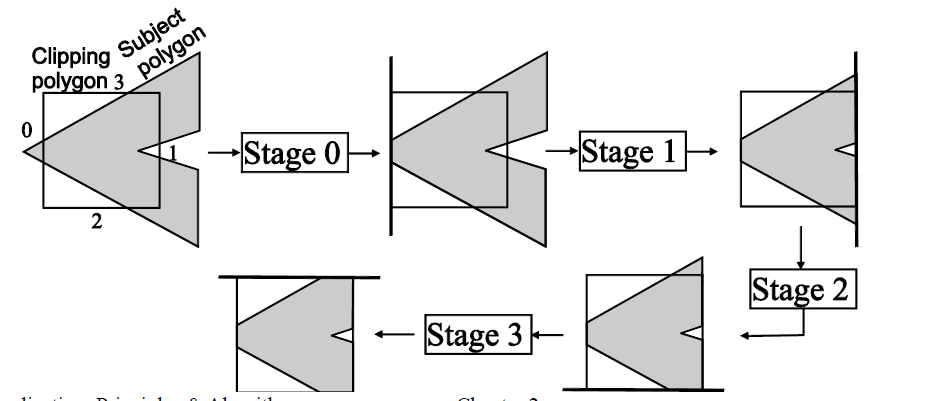
\includegraphics[width=\textwidth]{Bilder/sh.png}
Når man klipper en linje med en linje, kan man få forskjellige outputs. Se svart piksel:
\\ 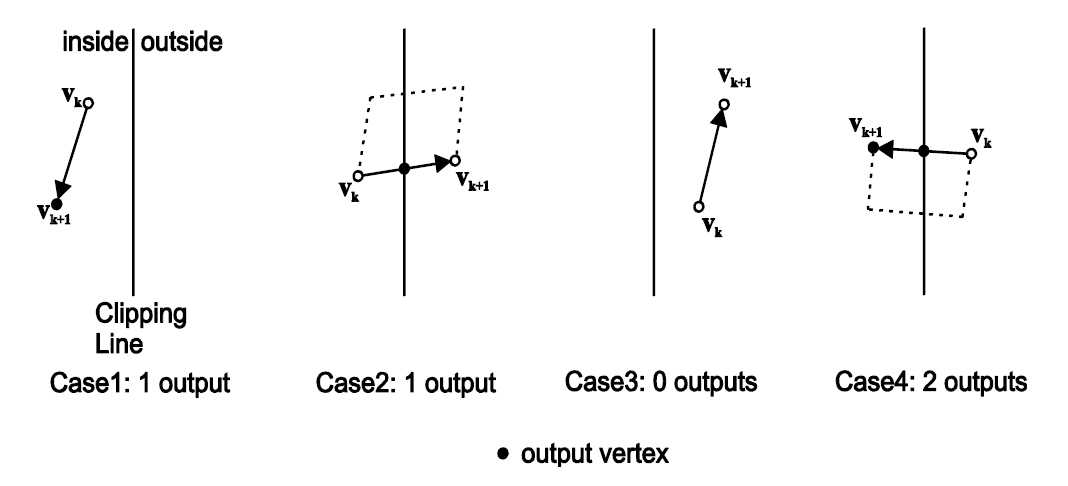
\includegraphics[width=\textwidth]{Bilder/sho.png}
Kompleksitet på SH er $O(mn)$ der $m$ er antall noder av klippepolygonet og $n$ er antall noder av subjektpolygonet.

\subsubsection{Greiner-Hornmann}
Støtter både clipping polygons og subject polygons
\begin{enumerate}
    \item Gå igjennom polygon S, og skru en bryter "av og på" når du kommer inn i C (bruk winding number).
    \item Gjør det samme med C med hensyn på S.
    \item Unionen av linjene som er tegnet opp er resultatet ditt
\end{enumerate}
Enkelt å regne ut $C \cup S$ ved å endre starttilstand på "av og på"-bryterne.

\subsection{Litt smått om koordinatsystemer og transformasjoner}
Gå fra 
\\ object coordinates $\rightarrow$ World coordinates $\rightarrow$ eye coordinates \\
Vi bruker høyrehånds koordinatsystemer. \\
En transformasjon er en mapping til og fra masse sett (f.eks. $E^3$ til $E^3$).

\subsection{Affine transformation}
Affine transformasjoner tar vare på affine kombinasjoner.
En kombinasjon av punkter er affin dersom:
\begin{equation}
    \vec{p} = \sum_{i=0}^n a_i \vec{p_i}
\end{equation}
og
\begin{equation}
    \sum_{i=0}^n a_i = 1
\end{equation}

En transformasjon er affin dersom den bevarer affine kombinasjoner, ergo:
\begin{equation}
    \Phi (\vec{p}) = \sum_{i=0}^n a_i \Phi (\vec{p_i})
\end{equation}
Konsekvenser av dette er at man bare trenger å regne ut "ekstremitetene" av polygoner.

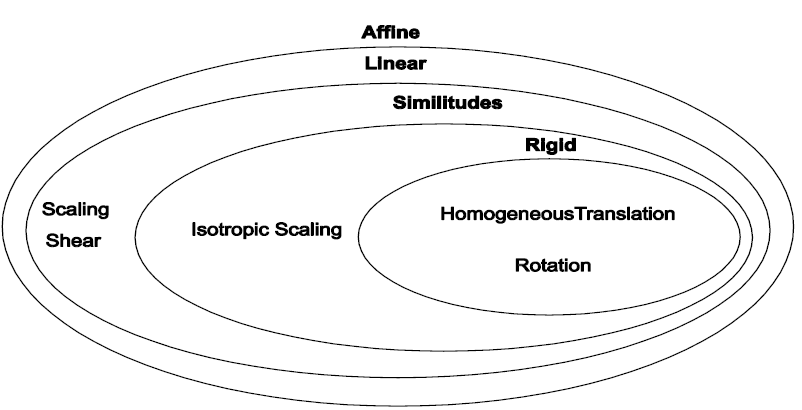
\includegraphics[width=\textwidth]{Bilder/Affine.PNG}

\subsection{Homogene koordinater}
Vi trenger dette, fordi forflytting av et punkt ikke kan uttrykkes som en lineær kombinasjon av x og y i et punkt. Vi innfører derfor en ekstra dimensjon, $w$ som ikke kan være $w=0$. \\
Når man bruker homogene koordinater unngår man også "fixed point", altså at en transformasjon på et punkt i origo alltid vil resultere i et nytt punkt i origo.

\subsection{Transformasjon i 3D}

\subsubsection{Translation}

\begin{equation} \label{eq:translation_matrix}
    \boldsymbol{T(\vec{d})} = 
   \begin{matrix}
        1 & 0 & 0 & d_x \\
        0 & 1 & 0 & d_y \\
        0 & 0 & 1 & d_z \\
        0 & 0 & 0 & 1
    \end{matrix}
\end{equation}
\begin{equation}
    \boldsymbol{T^{-1}(\vec{d}}) = \boldsymbol{T(-\vec{d})}
\end{equation}


\subsubsection{Scaling}

\begin{equation} \label{eq:scaling_matrix}
    \boldsymbol{S(s_x, s_y, s_z)} = 
   \begin{matrix}
        s_x & 0 & 0 & 0 \\
        0 & s_y & 0 & 0 \\
        0 & 0 & s_z & 0 \\
        0 & 0 & 0 & 1
    \end{matrix}
\end{equation}
\begin{equation}
    \boldsymbol{S^{-1}(s_x, s_y, s_z)} = \boldsymbol{S({1 \over s_x}, {1 \over s_y}, {1 \over s_z})}
\end{equation}

\subsubsection{Rotation}

\begin{equation}
    \boldsymbol{R_x}(\theta) =
    \begin{matrix}
        1 & 0 & 0 & 0 \\
        0 & cos(\theta) & -sin(\theta) & 0 \\
        0 & -sin(\theta) & cos(\theta) & 0 \\
        0 & 0 & 0 & 1
    \end{matrix}
\end{equation}

\begin{equation}
    \boldsymbol{R_y}(\theta) =
    \begin{matrix}
        cos(\theta) & 0 & sin(\theta) & 0 \\
        0 & 1 & 0 & 0 \\
        -sin(\theta= & 0 & cos(\theta) & 0 \\
        0 & 0 & 0 & 1
    \end{matrix}
\end{equation}

\begin{equation}
    \boldsymbol{R_z}(\theta) =
    \begin{matrix}
        cos(\theta) & -sin(\theta) & 0 & 0 \\
        sin(\theta) & cos(\theta) & 0 & 0 \\
        0 & 0 & 1 & 0 \\
        0 & 0 & 0 & 1
    \end{matrix}
\end{equation}

\begin{equation} \label{eq:rotation_inverse}
    \boldsymbol{R^{-1}}(\theta) = \boldsymbol{R}(-\theta)
\end{equation}    
Likning \ref{eq:rotation_inverse} gjelder alle rotasjonsmatriser.

\subsubsection{Shear}
\begin{equation}
    \boldsymbol{SH_{xy}}(a,b) =
    \begin{matrix}
        1 & 0 & a & 0\\
        0 & 1 & b & 0\\
        0 & 0 & 1 & 0\\
        0 & 0 & 0 & 1
    \end{matrix}
\end{equation}

\begin{equation}
    \boldsymbol{SH_{xz}}(a,b) =
    \begin{matrix}
        1 & a & 0 & 0\\
        0 & 1 & 0 & 0\\
        0 & b & 1 & 0\\
        0 & 0 & 0 & 1
    \end{matrix}
\end{equation}

\begin{equation}
    \boldsymbol{SH_{yz}}(a,b) =
    \begin{matrix}
        1 & 0 & 0 & 0\\
        a & 1 & 0 & 0\\
        b & 0 & 1 & 0\\
        0 & 0 & 0 & 1
    \end{matrix}
\end{equation}

For XY-shear blir x addert med a*z, og y addert med b*z.




\subsubsection{Change of basis}
Hvis du har tre ortonormale vektorer (alle står vinkelrett på hverandre, er enhetsvektorer (lengde=1), kan du endre fra gjeldende koordinatsystem til dette koordinatsystemet. Husk at begge systemene må ha samme "retning" (høyre- eller venstrehånd).

$$ \vec{i} = [a, b, c] $$
$$ \vec{j} = [d, e, f] $$
$$ \vec{k} = [p, q, r] $$

\begin{equation} \label{eq:basis_matrix}
    \boldsymbol{M_{BASIS}}=
    \begin{matrix}
        a & b & c & 0 \\
        d & e & f & 0 \\
        p & q & r & 0 \\
        0 & 0 & 0 & 1
    \end{matrix}
\end{equation}

\begin{equation}
    \boldsymbol{M^{-1}_{BASIS}} = \boldsymbol{M_{BASIS}^T} =
    \begin{matrix}
        a & d & p & 0 \\
        b & e & q & 0 \\
        c & f & r & 0 \\
        0 & 0 & 0 & 1
    \end{matrix}
\end{equation}

\subsection{Projeksjoner og sånn}
Vi tar koordinatsystemet gjennom: \\
World Cordinate system $\rightarrow$ Eye coordinate system $\rightarrow$ Canonical screen system.
\subsubsection{WCS to ECS}
Brukeren bestemmer her hva han vil se av verden, og gjør operasjoner som culling enklere.
\subsubsection{ECS til CSS}
Ta alle objekter som har overlevd inn i en kube (-1,-1,-1) til (1,1,1). Behold høy flyttalspresisjon. Herifra kan objektene lett taes opp på skjermer.

\subsubsection{Projeksjon}
Å ta noe fra 3D til 2D. To typer:
\begin{itemize}
    \item Perspective: Distansen mellom center of projection og projeksjonsplan er endelig.
    \item Parallell: Distansen mellom center of projection og projeksjonsplan er uendelig
\end{itemize}
Projeksjonsmappinger er ikke affine.

\subsubsection{Perspective projection}
\begin{equation} \label{eq:perspective_matrix}
    \boldsymbol{P_{PER}} =
    \begin{matrix}
        d & 0 & 0 & 0 \\
        0 & d & 0 & 0 \\
        0 & 0 & d & 0 \\
        0 & 0 & 1 & 0
    \end{matrix}
\end{equation}
(\ref{eq:perspective_matrix}) gjelder hvis planet står langs Z-aksen.

\subsubsection{Ortografisk projeksjon}
\begin{equation} \label{eq:orthographic_projection_matrix}
    \boldsymbol{P_{ORTHO}} =
    \begin{matrix}
        1 & 0 & 0 & 0 \\
        0 & 1 & 0 & 0 \\
        0 & 0 & 0 & 0 \\
        0 & 0 & 0 & 1
    \end{matrix}
\end{equation}
(\ref{eq:orthographic_projection_matrix}) fjerner effektivt z-koordinaten (punktene blir med andre ord projisert ned på xy-planet).

\subsubsection{Oblique Projection}
I stedet for å sende alle punkter ned med en vektor som står normalt på xy-planet (z-aksen), kan man sende dem med en retning $\vec{DOP}$ (Direction of projection). Vi får da:
\begin{equation}
    \vec{P'} = \vec{P} + \lambda \vec{DOP}
\end{equation}
Siden $P'_z$ = 0, får vi at $ \lambda = - {z \over DOP_z} $.
Av dette følger:
\begin{equation}
    \boldsymbol{P_{OBLIQUE}}(\vec{DOP}) =
    \begin{matrix}
        1 & 0 & -{DOP_x \over DOP_z} & 0 \\
        0 & 1 & -{DOP_y \over DOP_z} & 0 \\
        0 & 0 & 0 & 0 \\
        0 & 0 & 0 & 1
    \end{matrix}
\end{equation}

\subsubsection{Projeksjon ned på en hvilken som helst flate}
\begin{equation}
    \boldsymbol{P}=
    \begin{matrix}
        c & 0 & 0 & 0 \\
        0 & c & 0 & 0 \\
        0 & 0 & c & 0 \\
        n_x & n_y & n_z & 0
    \end{matrix}
\end{equation}
Her er $c = n_x x_0 + n_y y_0 + n_z z_0$. Utgangspunktet i utregningen er at $\vec{OP'} = a\vec{OP}$.

\subsection{WCS til ECS}
Nok informasjon for å definere ECS er $(\vec{E}, \vec{up}, \vec{g})$ der E er origo, $\vec{up}$ er retningen opp, $\vec{g}$ er synsretningen. Vi ønsker å ha det inn i følgende koordinatsystem:
\begin{itemize}
    \item $x_e$ er den horisontale aksen og øker til høyre.
    \item $y_e$ er den vertikale aksen og øker oppover.
    \item $z_e$ peker mot observatøren.
\end{itemize}
Regnes ut slik (lett å se for seg hvis man tegner det):
\begin{equation}
    \vec{z_e} = -\vec{g}
\end{equation}
\begin{equation}
    \vec{x_e} = \vec{up} \times \vec{z_e}
\end{equation}
\begin{equation}
    \vec{y_e} = \vec{z_e} \times \vec{x_e}
\end{equation}
Forflytt med $-\vec{E}$. Gjør alle disse vektorene om til enhetsvektorer og endre basis med matrise (\ref{eq:basis_matrix}).

\subsection{ECS til CSS}
\subsubsection{Ortografisk} \label{subsubsec:ortographic}
Tanken bak dette er at du har et paralellepiped som er definert med koordinatene (l,b,n) (left, bottom, near) og (r,t,f) (right, top, far). Dette skal mappes inn i (-1, -1, -1), (1, 1, 1).
\begin{enumerate}
    \item Flytt boksen din slik at midtpunktet er i origo med (\ref{eq:translation_matrix}): $\boldsymbol{T}(-{r+l \over 2}, -{t+b \over 2}, -{n+f \over 2})$
    \item Skalér slik at det får størrelse 2 med (\ref{eq:scaling_matrix}):
    $\boldsymbol{S}({2 \over r-l}, {2 \over t-b}, {2 \over f-n})$
\end{enumerate}

\subsubsection{Perspektiv}
Alt blir værre når det er snakk om perspektiv, men alt vi ønsker er å gjøre frustumet ("pyramiden") vår om til en parallelepiped slik at vi kan bruke ortografisk transformasjon fra ECS til CSS. Se bilde:
\\ 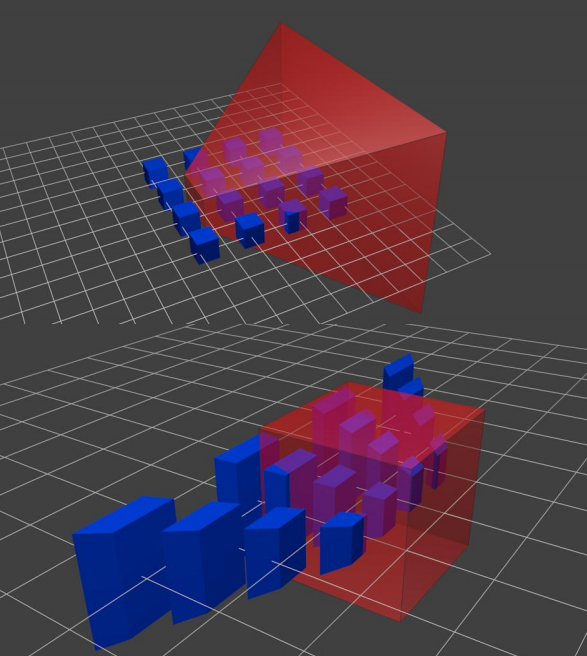
\includegraphics[width=\textwidth]{Bilder/projection_matrix.png}
Som man ser, kan vi ikke kvitte oss med z-koordinaten som i (\ref{eq:perspective_matrix}).
\\ Et slikt view blir definert med $\theta$, $z_e = n$, $z_e = f$ og $aspect$.

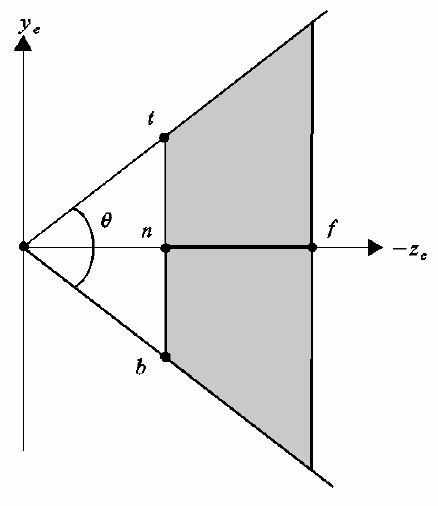
\includegraphics[width=\textwidth]{Bilder/perspective.PNG}

Regner ut:
\begin{equation}
    t = |n|tan({\theta \over 2})
\end{equation}
\begin{equation}
    b = -t
\end{equation}
\begin{equation}
    r = t*aspect
\end{equation}
\begin{equation}
    l = -r
\end{equation}

Vår nye z-koordinat blir: $z_s = A + {B \over z_e}$. Siden vi vet at $z_e=n$ må mappes til $z_s=n$ og $z_e=f$ må mappes til $z_s=f$, får vi følgende matrise:
\begin{equation}
    \boldsymbol{P_{VT}}=
    \begin{matrix}
        n & 0 & 0 & 0 \\
        0 & n & 0 & 0 \\
        0 & 0 & n+f & -nf \\
        0 & 0 & 1 & 0
    \end{matrix}
\end{equation}
Nå er det bare å fortsette med CSS-konverteringen som i \ref{subsubsec:ortographic}. Husk at matrisen kun gjelder hvis "pyramiden" ligger langs z-aksen, så du trenger ikke å forflytte boksen i x- og y-retning.

\subsubsection{Frustum culling}
Etter at vi har kommet i CSS, er det lett å sjekke om punkter er innenfor. Sørg for:
\begin{equation} \label{eq:frustum_culling}
    -w \le x, y, z \le w
\end{equation}

\subsubsection{Hvorfor klippe i 3D og ikke i 2D?}
\begin{itemize}
    \item I vanlig perspektivprojeksjon vil objekter på baksiden av $E$ bli opp-ned (vi mister informasjon om klipping).
    \item Unngår potensielt perspektiv-deling på null.
    \item Blir lettere å allokere dybdebuffer, når vi vet at alle z-verdiene er mellom -1 og 1.
\end{itemize}

\subsubsection{What happens next?}
CSS flyttes til viewport coordinate system med først en skalering, så en forflytning.



\subsection{Hidden Surface Elimination}
To måter.

O($P^2$):
\begin{lstlisting}
for each primitive {
    find visible part
    render visible part
}
\end{lstlisting}

O($Pp$):
\begin{lstlisting}
for each pixel {
    find closest primitve
    render pixel with color of closest primitve
}
\end{lstlisting}
Dette er tunge operasjoner. Mye kan fjernes.
\begin{itemize}
    \item Fjerne baksidepolygoner (back-face culling)
    \item Fjerne elementer som er helt på utsiden av frustum (frustum culling)
\end{itemize}
Siden dette har kjøretid på enten $O(P)$ eller $O(Pv)$ (v er average number of vertices per primitive), ser vi at flaskehalsen er HSE-algoritmene.

\subsection{Back-face culling}
Enkel operasjon. Hvis $\vec{g}$ er syssretningen og $\vec{n}$ er normalvektoren til et polygon, elliner alle som står mindre enn 90 grader på synsretningen.
\begin{equation}
    \vec{g} \cdot \vec{n} > 0
\end{equation}

\subsection{Frustum culling}
Som beskrevet i likning (\ref{eq:frustum_culling}). \\
Siden punkter ikke har konstant $w$, må denne interpoleres med
\begin{equation}
    (1-t) w_1 + t w_2
\end{equation}
Ulikhetene må også skrives om:
\begin{equation}
    -((1-t)w_1 + t w_2) \le (1-t)x_1 + t x_2 \le (1-t)w_1 + t w_2
\end{equation}
\begin{equation}
    -((1-t)w_1 + t w_2) \le (1-t)y_1 + t y_2 \le (1-t)w_1 + t w_2
\end{equation}
\begin{equation}
    -((1-t)w_1 + t w_2) \le (1-t)z_1 + t z_2 \le (1-t)w_1 + t w_2
\end{equation}

\subsection{3d clipping}
Algoritmene beskrevet i \ref{subsection:clipping} kan utvides til 3D.

For Cohen-Sutherland, utvid med to ekstra bits for z-verdier. Triviell aksept og triviell forkastning vil fortsatt fungere.

\subsection{Z-buffer algorithm}
Veldig enkel algoritme. Grafikkort har, sammen med sitt display-buffer, tilknyttet et z-buffer med 1:1-korresponsdanse mellom piksler.
\begin{enumerate}
    \item Initier z-bufferet med verdien til "far clipping plane".
    \item For hver piksel som skal tegnes, sjekk z-bufferet. Hvis z-verdien i bufferet er større enn pikselen som skal tegnes, oppdater både display- og z-buffer.
\end{enumerate}

Siden det er strevsomt å regne ut ny z-verdi for hver x- og y-verdi, tar man i bruk fremoverdifferanser.
\begin{equation}
    F(x,y) = z = - {d \over c} - {a \over c}x - {b \over c}y
\end{equation}
Utledet fra den implisitte likningen for et plan. Fremoverdifferansen for x blir da
\begin{equation}
    F(x+1,y)-F(x,y) = - {a \over c}
\end{equation}
Dette gjør det lettere å regne ut z, trenger bare én addisjon per steg.

I praksis blir z-verdi interpolert ut ifra z-verdier på kantene til et polygon. Komplkisiteten til algoritmen en $O(Ps)$ hvor s er gjennomsnittlig antall piksler dekket av et polygon. Dette er en veldig enkel algoritme, men den sliter med transparente objekter.

\subsection{Bounding volumes}
Mange komplekse polygoner kan gjøre det dyrt med beregninger av linjekrysninger. Man kan da bruke bounding boxes, selv om de kan gi falsk alarm på grunn av void space. Men du kan vite at de går klar av hverandre hvis bounding-boksene går klar av hverandre.

Man vil ha minst mulig void space. Mulige løsninger:
\begin{itemize}
    \item Lage parallelpiped som bounding box.
    \item Orienterte parallelepipeds.
    \item Hiearkiske bounding-bokser.
    \item Progressive hulls. Polygoner som er enkle, som blir "vanskeligere" jo større oppløsning man trenger. Man kommer til slutt til de faktiske polygonene og kan da beslutte.
\end{itemize}

\subsubsection{Space subdivision}
Deles opp i celler. Der scenene er enkle, er cellene store, men blir mindre ved behov. Minste størrelse er en voxel.

\subsection{Illuminering}
En illumineringsmodell belyser punkt p og tar høyde for mye:
\begin{itemize}
    \item Direction of light
    \item Directon of observation
    \item Surface normal
    \item Materialegenskaper
    \item mye mer....
\end{itemize}
Dette skjer etter at objektene har fått teksturer. Lyset $i$ som beregnes skalerer fargevektoren. \\
Forskjell på illumination model og illumination algorithm. Sistnevnte implementerer en modell i en effektiv algoritme.

\subsection{Phong Illumination Model}
Denne modellen gjør om innkommende lys med styrke og vinkel $(\Theta_i, \phi_i)$ til utgående lys $(\Theta_i, \phi_i)$ for et punkt $\vec{p}$. Tar ikke høyde for lys som er reflektert fra andre kilder. Fire komponenter:

\begin{itemize}
    \item Emmision
    \item Ambient reflection
    \item Diffuse reflection
    \item Specular reflection
\end{itemize}

\subsubsection{Emmision $I_e$}
For objekter som er selvlysende.

\subsubsection{Ambient $I_g$}
Gjør slik at en overflate uten direkte lys synes likevel. Hele scenen har $I_a$, konstant ambient light, som gjør:
\begin{equation}
    I_g = I_ak_a
\end{equation}
$k_a$ er da ambient reflectance coefficient.

\subsubsection{Diffuse $I_d$}
Lys som blir spredt i alle retninger, proposjonalt med vinkelen lyset treffer punktet på.
\begin{equation} \label{eq:phong_diffuse}
    I_d = I_ik_dcos\theta = I_ik_d(\vec{n}\cdot\vec{l})
\end{equation}
Her er $\theta$ vinkelen mellom normalvektoren til pikselen og retningen på lyset. Disse må være enhetsvektorer for at (\ref{eq:phong_diffuse}) skal stemme.

Det er også mulig å ha forskjellige $k_d$ for ulike bølgelengder, altså ulike fargeverdier.

\subsubsection{Specular $I_s$}
Her er det sammenheng mellom vektoren fra lyset til punktet og fra kamera til punktet.
\begin{equation}
    I_s = I_ik_s cos^n\alpha = I_ik_s(\hat r\cdot \hat v)^n
\end{equation}
Her er $\hat r$ vektoren som reflekteres av punktet for lyskilden. Vi ser at i jo større grad kameraretningen $\hat v$ samsvarer med $\hat r$, jo kraftigere lys. For at lyset skal avta fortere, og vi får mer "shinyness", legger vi på en eksponent $n$. Jo høyere $n$, jo mindre spredning, og mer "shininess".\\
Specular reflection tar fargen til lyskilden, ikke til objektet selv.

\subsubsection{Sammenheng mellom diffuse og specular}
Specular og diffuse henger tett sammen. Koeffisientene henger tett sammen:
\begin{equation}
    0 \le kd,ks \le 1, kd + ks \le 1
\end{equation}
Diffuse tilsvarer matte overflater, specular glatte overflater.

\subsubsection{Distance factor}
En tilnærming til avtagende lys, der lyset blir svakere jo lenger unna du er. En modell med tre konstanter ser ut som dette:
\begin{equation}
    f(d) = {1 \over c_1 + c_2d + c_3d^2}
\end{equation}
Funksjonen multipliseres med specular- og diffuse-leddene i 

\subsubsection{Fargeavhengighet}
Man kan forskjellige koeffesienter for R, G og B. Dette gjelder ikke specular lightning, da dette skal simulere en hvit lyskilde.

\subsubsection{Vektorer brukt i Phong}
Vi trenger følgende vektorer for å beregne lysverdier:
\begin{itemize}
    \item $\vec{n}$
    \item $\vec{l}$
    \item $\vec{n}$
    \item $\vec{r}$ eller $\vec{h}$
\end{itemize}

\paragraph{Normalvektor}
Normalvektoren til en implisitt overflate er gradienten til overflaten.
\begin{equation}
    \vec{n} = \nabla f(x,y,z)
\end{equation}
For likningen for et plan forenkles dette til:
\begin{equation}
    \vec{n} = [a,b,c]^T
\end{equation}
For en parametrisk variant har vi følgende:
\begin{equation}
    \begin{aligned}
        x = f_x(u,v) \\
        y = f_y(u,v) \\
        z = f_z(u,v)
    \end{aligned}
\end{equation}
Normalvektoren blir da
\begin{equation}
    \vec{n} = {\vec{\partial f} \over \vec{\partial u}} \times
    {\vec{\partial f} \over \vec{\partial v}}
\end{equation}

Ofte vet vi bare nodene, ikke likningene. Bruk ordinært kryssprodukt for tre noder. Dersom man har flere noder som ikke er i plan, må man approksimere normalvektoren. Dette kan man gjøre ved hjelp av gjennomsnitt eller en metode som heter Martin-Newell's teknikk.

\paragraph{Martin-Newell's teknikk}
\begin{equation}
    \vec{n} = \begin{bmatrix}
        \sum_{i=1}^n(y_i - y_{i\oplus 1})(z_i + z_{i\oplus 1}) \\
        \sum_{i=1}^n(z_i - z_{i\oplus 1})(x_i + x_{i\oplus 1}) \\
        \sum_{i=1}^n(x_i - x_{i\oplus 1})(y_i + y_{i\oplus 1})
    \end{bmatrix}
\end{equation}

\paragraph{Nodenormaler}
Kan være greit å ha normaler per node, og ikke bare for overflatene (hvis man skal runde av kantene. Her kan man ta snittet av normalvektorene til polygonene som inneholder den gitte noden. Man kan også vekte normalvektorene, der de større bidrar mer. En siste metode er å la vinkelen bestemme hvor mye normalvektoren skal telle. Jo større vinkel, jo mer bidrag.


\paragraph{Refleksjonsvektorer}

Refleksjonsvektoren regnes ut som dette:
\begin{equation}
    \vec{r} = 2 \vec{r_1} - \hat l = 2 \hat n(\hat n \cdot \hat l) - \hat l
\end{equation}
\\ 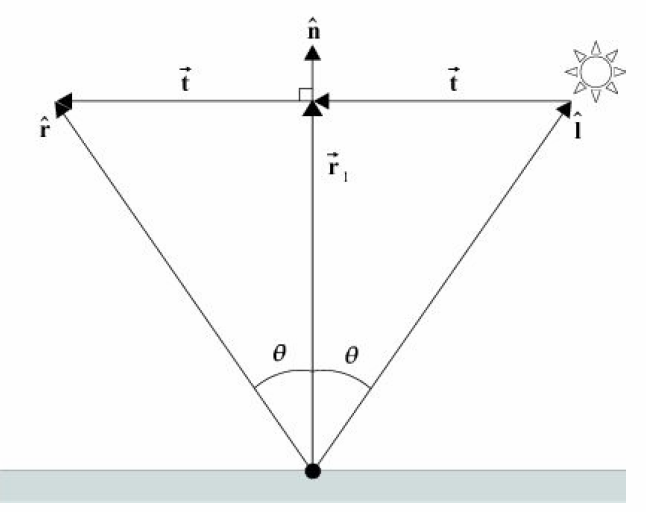
\includegraphics[width=\textwidth]{Bilder/reflection.png}

\subsection{Illumination algorithms}
Algoritmene bruker en illuminasjonsmodell og gjennomfører utregningene.
\subsubsection{Constant shading}
\begin{itemize}
    \item Ingen specular reflection
    \item Lys- og kamera er plassert samme sted, og uendelig langt borte.
    \item $\hat n \cdot \hat l$ er konstant for hvert polygon
\end{itemize}

\subsubsection{Gouraud Shading}
\begin{itemize}
    \item Regner ut intensiteter per node.
    \item Interpolerer kantene med lineær sammenheng mellom lystyrkene på hver side.
    \item Interpolerer hver scanline med verdiene regnet ut på kantene i punktet ovenfor.
\end{itemize}

\subsubsection{Phong Shading}
\begin{itemize}
    \item Regner ut en ny lysstyrke for hver piksel
    \item Regner i stedet ut normalvektorene med interpolasjon (som beskrevet i Gouraud Shading)
\end{itemize}

\subsection{Grayscale}
For å representere akromatisk lys (gråtone), er lineære intensiteter en dårlig idé, siden øyet vårt ikke fungere på den måten. Vi opererer heller med ratioer mellom påfølgene lysverdier.

\begin{equation}
    \begin{aligned}
    \Phi_1 = \lambda * \Phi_0 \\
    \Phi_2 = \lambda * \Phi_1 = \lambda^2*\Phi_0 \\
    \dots \\
    \Phi_{n-1} = \lambda^{n-1} * \Phi_0 = 1
    \end{aligned}
\end{equation}
    

\subsection{Gamma Correction}
Skjermer har et ikke-lineært forhold mellom input- og output-verdier. Gamma-correction er å justere input-verdiene slik at vi får et lineært forhold:
\begin{equation}
    input' = input^{1 \over \gamma}
\end{equation}

\subsection{Color model}
En mdell for å kunne gjøre følgende med farger:
\begin{itemize}
    \item Beskrive
    \item Sammenligne
    \item Klassifisere
    \item Sortere
\end{itemize}
Vi har både deviceavhengige og deviceuavhengige modeller.\\
I en deviceuavhnegig modell vil en fargekoordinat representere en unik farge, og er nyttig for å konvertere mellom deviceavhengige modeller

\subsubsection{Perceptual linearity}
Forskjellen mellom to farger er propesjonal med forskjellen i fargeverdiene i fargemodellen.

\subsection{CIE XYZ Color Model}
Beskriver faktiske farger med bølgelengder.
\\ 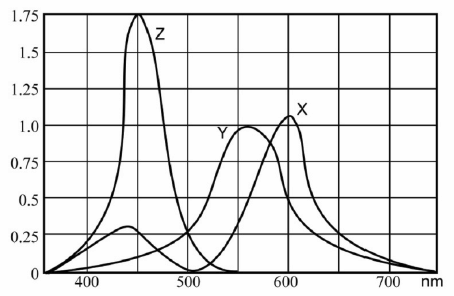
\includegraphics[width=\textwidth]{Bilder/cie.png}
X,Z inneholder informasjon om farge, mens Y inneholder lysstyrke.

\subsection{RGB Color Model}
Additiv modell som begynner med svart og ender i hvit. Den er god på grunn av sin additive natur og at RGB er synlige farger, ikke teoretiske kvantiteter. Ikke perceptually linear, det er vanskelig å "finne opp" en hvilken som helst farge.

\subsubsection{RGB Cube}
Enhetskube med alle farger i RGB-modellen. Retning på vektor bestemmer chromaticity, lengde er intensitet.

\subsubsection{RGB Triangle}
Du kan mappe alle farger i en triangel med hjørner (1,0,0), (0,1,0) og (0,0,1), eneste du mister er intensitet. Ved å bruke denne triangelen kan vi få nye begreper:
\begin{itemize}
    \item Hue. Den dominerende bølgelengden.
    \item Saturation. Hvor mye vitt som er i en farge.
\end{itemize}

\subsection{HSV Color model}
Deler opp i Hue, Saturation og Intensity i en kjegle Hue er et fargehjul, hvor vinkelen bestemmer farge. Jo lenger ut på kantene du kommer til hjulet, jo høyere saturation. Høyest intensitet på bunnen av kjeglen, lavest på toppen (spissen)

\subsection{CMY Color model}
Invers av RGB. Er substraktiv, bra for printere (som begynner på hvit og gjør ting mørkere). CMYK legger på en svart komponent, for bedre sortkvalitet på skrivere.

\subsection{High Dynamic Range}
Dynamisk rekkevide til et bilde er ratioen fra høyeste til laveste intensitetsverdi. Et vanlig RGB-bilde har en dynamisk rekkevidde på 90:1, øyet har på 10'000:1. Et vanlig RGB-bilde gjør en god jobb med å vise hva en monitor kan, men ikke hva et øye kan. For å lage HDR-bilder kan man for eksempel ta flere bilder med ulik eksponeringstid og sette sammen.







